% Main Presentation File
\documentclass{beamer}
\usepackage{listings}

\usepackage[utf8]{inputenc}

\lstset{
    language=Python,
    basicstyle=\ttfamily\scriptsize,
    breaklines=true,
    frame=single,
    numbers=none,
    keywordstyle=\color{red}\bfseries,
    stringstyle=\color{green!60!black},
    commentstyle=\color{gray},
    showstringspaces=false,
    columns=flexible,
    backgroundcolor=\color{gray!10},
}

\usetheme{CambridgeUS}

\title{Coordination of a Multi-Agent System for Emergency Response}
\author{Team 05}
\date{\today}

\begin{document}


% Slide 1: Title Slide
\title{Coordination of a Multi-Agent System \\for Emergency Response}
\author{Team 05}
\date{\today}

\begin{frame}
    \titlepage
\end{frame}


% Slide 2: Overview of the Project
\begin{frame}{Overview}
    \begin{itemize}
        \item Task 1 focused on environment and agent design
        \item Task 2 explored coordination mechanisms
        \item Now, we integrate these into a practical implementation
        \item Implementation utilizes \textbf{CrewAI} and \textbf{Ollama}
        \item In this presentation, we will cover:
        \begin{itemize}
            \item Agents and their tasks
            \item Crews module and data models
            \item Database and tools
            \item Scripts
            \item Testing
            \item Integration in \texttt{main.py} and \texttt{data/} folder
        \end{itemize}
    \end{itemize}
\end{frame}


% Slide 3: Agents and Tasks
\begin{frame}[fragile]{\texttt{Agents and Tasks}}
    \begin{itemize}
        \item For each crew, we define agents and tasks using \texttt{.yaml} files.
        \item Each crew is represented as a Python class, with agents and tasks defined as methods within the class.
        \item Agents are instantiated with configuration settings, and tasks are created by linking them with specific tools and data models.
    \end{itemize}
      \begin{columns}
        \begin{column}{0.48\textwidth} % 48% width for the first listing
            \centering% Disable label for this listing
  \texttt{medical\_services/agents.yaml}
            \begin{lstlisting}[language=yaml]
hospital_coordinator:
  role: Hospital Coordinator
  goal: >
    ...
  backstory: >
    ...
  allow_delegation: false
  verbose: true
  llm: ollama/llama3.1
  temperature: 0.4
  max_tokens: 800

            \end{lstlisting}
        \end{column}
        \begin{column}{0.48\textwidth} % 48% width for the second listing
            \centering
              \texttt{medical\_services/tasks.yaml}
            \begin{lstlisting}[language=yaml]
rank_hospitals:
  description: >
  ...
  expected_output: >
  ...
  agent: hospital_coordinator
  context:
    - fetch_hospital_information
            \end{lstlisting}
        \end{column}
      \end{columns}
\end{frame}

% Slide 4: Crews Module
\section*{Crews Module}
\begin{frame}[fragile]{\texttt{src/emergency\_planner/crews/}}
    \begin{columns}[c]
      \begin{column}{0.3\textwidth}
          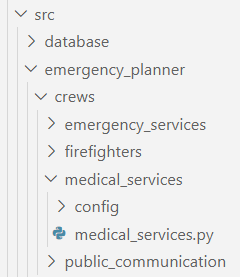
\includegraphics[width=\textwidth]{figures/crews_modules_folders.png}
      \end{column}
      \begin{column}{0.68\textwidth}
        \centering
        \texttt{medical\_services.py}
        \begin{lstlisting}[language=Python, breaklines=true]
@CrewBase
class MedicalServicesCrew:
    """Medical Services Crew"""
    @agent
    def medical_services_operator(self) -> Agent:
        return Agent(config=self.agents_config["medical_services_operator"])
        ...
    @task
    def fetch_hospital_information(self) -> Task:
        config = add_schema_to_task_config(
            self.tasks_config["fetch_hospital_information"],
            HospitalsInformation.model_json_schema(),
        )
        return Task(config=config, tools=[hospital_reader_tool])
        \end{lstlisting}
      \end{column}
    \end{columns}
\end{frame}

% Slide 5: Data Models
\begin{frame}[fragile]{\texttt{src/emergency\_planner/data\_models/}}
  \begin{columns}[c]
    \begin{column}{0.3\textwidth}
        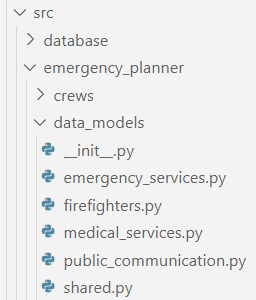
\includegraphics[width=\textwidth]{figures/data_models_folder.png}
    \end{column}
    \begin{column}{0.68\textwidth}
      \texttt{shared.py}
      \begin{lstlisting}[language=Python, breaklines=true]
FireType = Literal["ordinary",..., "other"]
FireSeverity = Literal["low", "medium", "high"]
... 
def add_schema_to_task_config(task_config, schema):
   ...
    return task_config
      \end{lstlisting}
      \texttt{public\_communication.py}
      \begin{lstlisting}[language=Python, breaklines=true]
from pydantic import BaseModel
from .shared import FireSeverity, FireType
from .medical_services import MedicalResponseReport
...
class EmergencyReport(BaseModel):
  medical_response_report: MedicalResponseReport
  fire_type: FireType
  fire_severity: FireSeverity
  ...
      \end{lstlisting}
    \end{column}
  \end{columns}
\end{frame}

% Slide 6: Database and Tools
\begin{frame}{Database and Tools}
    \vspace{2cm}
\end{frame}

% Slide 7: GPS Tools
\begin{frame}{GPS Tools}
    \vspace{2cm}
\end{frame}

% Slide 8: Scripts
\begin{frame}{Scripts}
    \vspace{2cm}
\end{frame}

% Slide 9: Test Script
\begin{frame}{Test Script}
    \vspace{2cm}
\end{frame}

% Slide 10: Test Folder
\begin{frame}[fragile]{\texttt{src/emergency\_planner/test/}}
    \begin{columns}
        \begin{column}{0.33\textwidth}
            \begin{figure}
                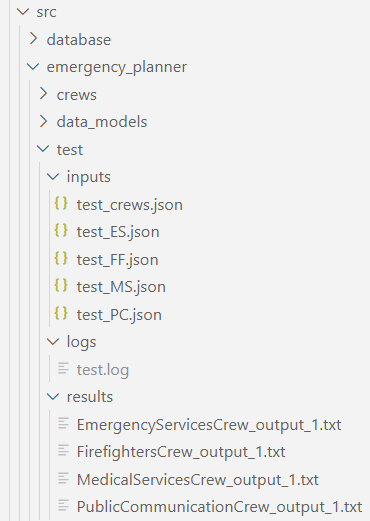
\includegraphics[width=\textwidth]{figures/test_folder_structure.png}
            \end{figure}
        \end{column}
        \begin{column}{0.67\textwidth}
            \centering
            \texttt{test\_crews.json}
            \begin{lstlisting}[language=json]
{
    "test_cases": [
        {
            "crew_to_test": "EmergencyServicesCrew",
            "crew_inputs": {
                "transcript": 
                    "A fire of electrical..."
            }
        }
    ]
    ...
}    
            \end{lstlisting}
        \end{column}
    \end{columns}
\end{frame}

% Slide 11: Integration in main.py
\begin{frame}[fragile]{\texttt{emergency\_planner/main.py}}
    \begin{lstlisting}[language=Python]
class EmergencyPlannerFlow(Flow[EmergencyPlannerState]):
    @start()
    def get_call_transcript(self): ...

    @listen(get_call_transcript)
    def emergency_services(self): ...

    @listen(emergency_services)
    def firefighters(self): ...

    @listen(emergency_services)
    def medical_services(self):
        if not self.state.call_assessment.medical_services_required:
            return
        ...
    
    @listen(or_(and_(firefighters, medical_services), "retry_public_communication"))
    def public_communication(self): ...
    
    @router(public_communication)
    def check_approval(self): ...
\end{lstlisting}
\end{frame}

% Slide 12: Integration Folder: data
\begin{frame}[fragile]{\texttt{data/}}
    \begin{columns}
        \begin{column}{0.33\textwidth}
            \begin{figure}
                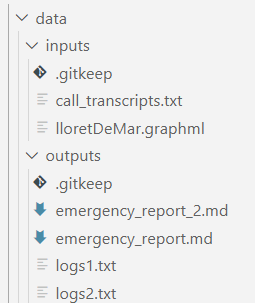
\includegraphics[width=\textwidth]{figures/data_folder_structure.png}
            \end{figure}
        \end{column}
        \begin{column}{0.67\textwidth}
        
    
            \begin{lstlisting}[language=Python]
@start()
def get_call_transcript(self):
    with open(EMERGENCY_CALL_TRANSCRIPTS_FILENAME, "r") as f:
        self.state.call_transcript = f.readlines()[TRANSCRIPT_INDEX]
            \end{lstlisting}
            \begin{lstlisting}[language=Python]
@listen("save full emergency report")
def save_full_emergency_report(self):
    full_emergency_report = f"""
# Emergency Report

## Call Transcript
{self.state.call_transcript}
...
"""
with open(EMERGENCY_REPORT_FILENAME, "w") as f:
    f.write(full_emergency_report)
            \end{lstlisting}
        \end{column}
    \end{columns}
\end{frame}

\end{document}
